\documentclass[conference]{IEEEtran}
\IEEEoverridecommandlockouts
% The preceding line is only needed to identify funding in the first footnote. If that is unneeded, please comment it out.
\usepackage{cite}
\usepackage{amsmath,amssymb,amsfonts}
\usepackage{algorithmic}
\usepackage{graphicx}
\usepackage{textcomp}
\usepackage{xcolor}
\def\BibTeX{{\rm B\kern-.05em{\sc i\kern-.025em b}\kern-.08em
    T\kern-.1667em\lower.7ex\hbox{E}\kern-.125emX}}
\begin{document}

\title{Relatório 4: Incrementação da multiplicação na ULA do MIPS\\}

\author{\IEEEauthorblockN{André Luiz Dal Vesco}
\IEEEauthorblockA{\textit{Engenharia Eletrônica} \\
Florianópolis, Brasil \\
andreluiz.dalvesco@gmail.com\\}
\and
\IEEEauthorblockN{Carlos Augusto Porto Freitas}
\IEEEauthorblockA{\textit{Engenharia Eletrônica} \\
Florianópolis, Brasil \\
caftrabalho@gmail.com\\}
\and
\IEEEauthorblockN{Giulia Donini Burkle}
\IEEEauthorblockA{\textit{Engenharia Eletrônica} \\
Florianópolis, Brasil \textcolor{white}{.................}  \\
giuliadoninib@gmail.com\\}
\and
\IEEEauthorblockN{Henrique Gonçalves de Medeiros}
\IEEEauthorblockA{\textit{Engenharia Eletrônica} \\
Florianópolis, Brasil \\
steamhique@gmail.com\\}
\and
\IEEEauthorblockN{João Victor Martins Conzatti}
\IEEEauthorblockA{\textit{Engenharia Eletrônica} \\
Florianópolis, Brasil \\
joaovictorconzatti@hotmail.com}
\and
\IEEEauthorblockN{Lucas Patrocinio Barreto Alves}
\IEEEauthorblockA{\textit{Engenharia Eletrônica} \\
Florianópolis, Brasil \\
lucas.patrocinio3003@gmail.com}
}

\maketitle

\begin{abstract}
O relatório em questão trata da otimização da Unidade Lógica e Aritmética (ULA) no contexto da arquitetura MIPS, especificamente no que diz respeito à implementação da instrução de multiplicação. A metodologia adotada inclui a implementação da arquitetura original da ULA com a modificação de uma saída de 64 bits, e além disso, a adição de uma nova instrução de multiplicação. Esta última emprega componentes adicionais e se caracteriza por um comportamento cíclico de adição, visando aprimorar a eficiência do sistema. Para avaliação da solução proposta, foi desenvolvido um testbench que contempla entradas representativas de valores críticos, juntamente com suas respectivas saídas e códigos de erro. Adicionalmente, foram conduzidos simulações e testes da arquitetura por meio do ModelSim. A análise do funcionamento e das estratégias implementadas para essa otimização compreende a avaliação dos resultados da síntese e das simulações, englobando parâmetros como atraso, entradas e saídas, e ocupação da placa. Os resultados obtidos evidenciam o funcionamento das instruções originais do MIPS, porém, sem sucesso na implementação da instrução de multiplicação. A utilização do ModelSim para simulações e testes contribuiu para a avaliação do funcionamento de certas partes da arquitetura. Em conclusão, este relatório apresenta uma implementação da ULA original do MIPS, e uma tentativa da implementação da instrução de multiplicação, que ocorreu sem sucesso.

\end{abstract}

\begin{IEEEkeywords}
MIPS, multiplicação, ULA, instrução
\end{IEEEkeywords}

\section{Introdução}
Esse relatório traz a incrementação da instrução de multiplicação na Unidade Lógica e Aritmética (ULA) na arquitetura MIPS. Inicialmente, será apresentado o modelo da arquitetura, os componentes utilizados e a máquina de estados, trazendo as diferenças e modificações em cima da ULA original, e seu funcionamento no geral. Então, será tratado da verificação da proposta por meio de um testbench e simulações, assim como os resultados da síntese do projeto à nível de consumo e espaço. 

\section{Proposta}

\subsection{Modelo da arquitetura}
Para comportar a instrução de multiplicação de forma eficaz, foi necessário alterar a quantidade de bits da saída da ULA de 32 bits à 64 bits, e com isso, separando a saída em dois registradores de 32 bits: high e low. Portanto, mesmo os componentes das instruções originais do MIPS tiveram que ser alterados para comportar o novo número de bits.

\begin{figure}[htbp]
\centerline{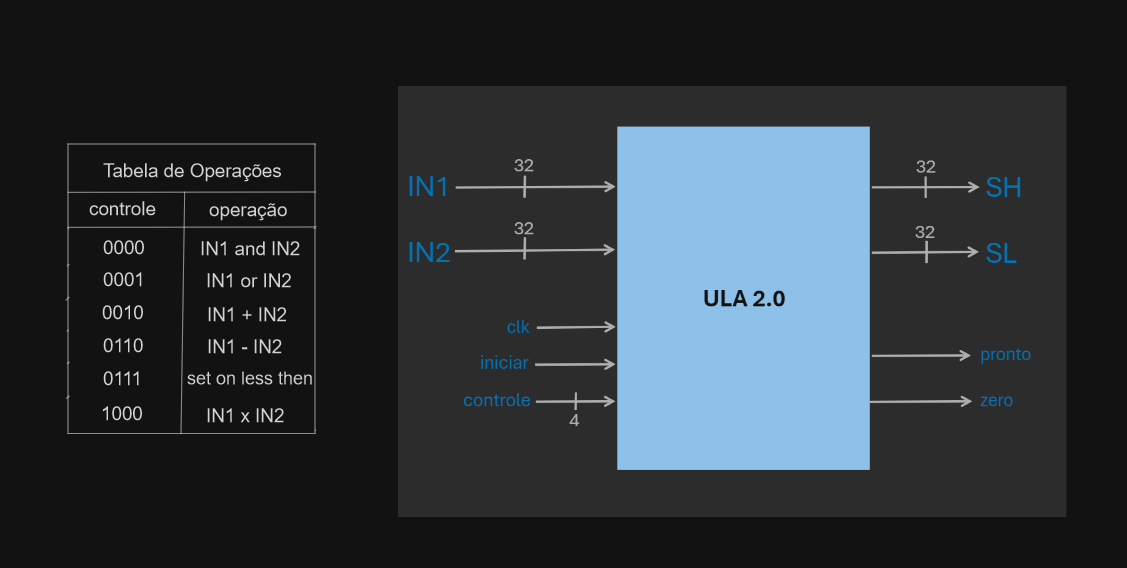
\includegraphics[scale=0.3]{ula_interface.png}}
\caption{Interface da ULA 2.0.}
\label{fig}
\end{figure}

O sinal de controle da ULA define qual instrução será realizada dentre as 6 opções, as quais serão explicadas a seguir.
\begin{itemize}
    \item IN1 and IN2 (0000): realiza um AND bit a bit nas entradas;
    \item IN1 or IN2 (0001):  realiza um OR bit a bit nas entradas;
    \item IN1 + IN2 (0010): realiza uma soma entre as entradas;
    \item IN1 - IN2 (0110): realiza a subtração da entrada 1 pela entrada 2;
    \item Set On Less Than (0111): define a saída como 1 caso IN1 seja menor que IN2;
    \item IN1 x IN2 (1000): realiza a multiplicação entre as entradas.
\end{itemize}

As primeiras 5 instruções são realizadas da mesma maneira que o MIPS convencional, apenas com um número diferente de bits. Por isso, será tratado mais a fundo do funcionamento da instrução de multiplicação, que é a principal implementação do projeto.

\begin{figure}[htbp]
\centerline{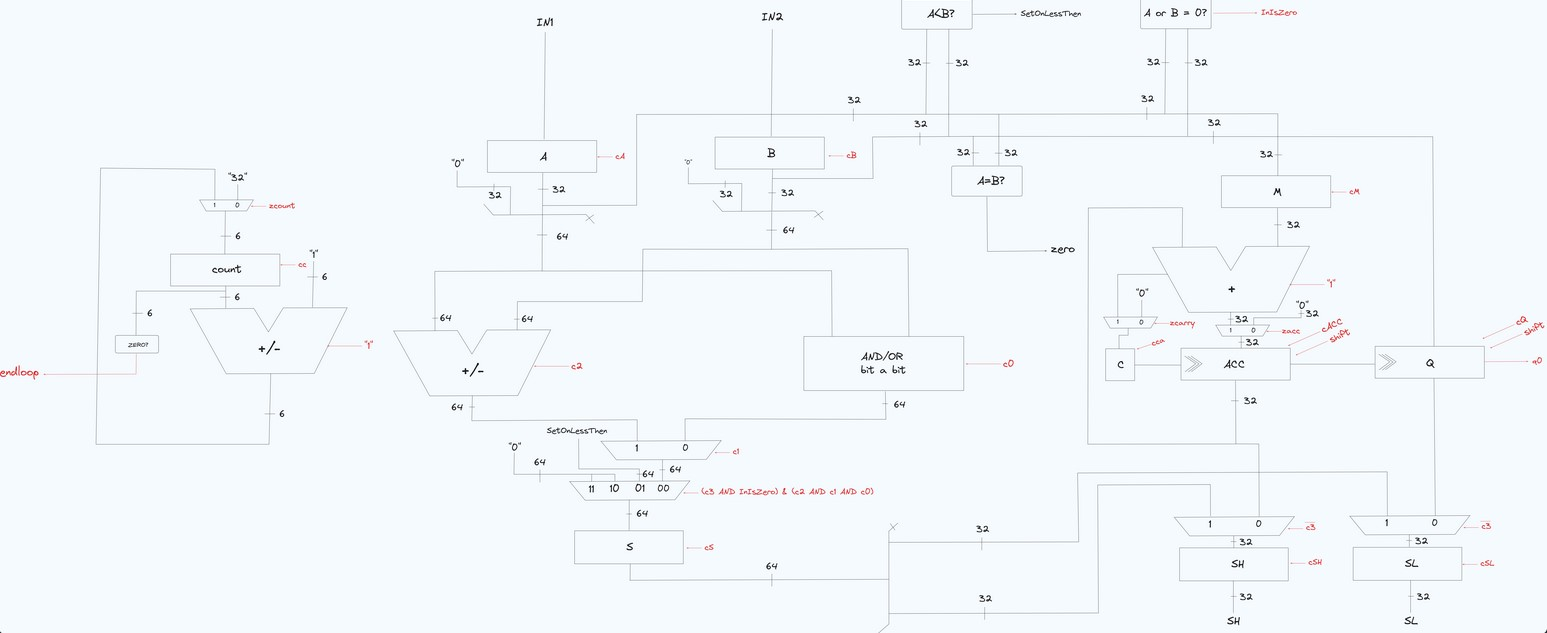
\includegraphics[scale=0.2]{ula_datapath.jpg}}
\caption{Datapath da ULA 2.0.}
\label{fig}
\end{figure}

À esquerda da figura 2, temos a estrutura de um contador utilizado para o ciclo de adições para a realização da multiplicação, que irá passar por todos os 32 bits das entradas, decrementando de 32 à 0, independente do valor das entradas.

À direita, temos a implementação em si da multiplicação. Primeiramente, a entrada IN1 é armazenada no registrador A e a entrada IN2 é armazenada no registrador B. Há uma comparação entre as duas entradas, a fim de verificar se uma delas é zero, e caso seja, o resultado será zero também, sem passar pelos outros componentes. Caso ambas entradas sejam diferentes de zero, temos o registrador M recebendo o valor de A, e o registrador de deslocamento Q recebendo o valor de B, e ACC será iniciado em 0. Ciclicamente, caso o bit menos significativo de Q seja igual à '1', o acumulador receberá o resultado da soma entre o valor anterior contido nele mesmo e o valor contido em M, e o registrador de deslocamento Q receberá o valor de carry, e então, este sofrerá um shift para a direita em uma casa, assim como o ACC. Caso o bit menos significativo de Q seja igual à '0', apenas os shifts serão executados, sem que haja a adição. Ao término da contagem de 32, os registradores SH e SL irão receber o resultado da multiplicação.

\subsection{Componentes}

\subsubsection{Multiplexadores}
A arquitetura da ULA 2.0 conta com sete multiplexadores em seu datapath. Para as instruções padrões, é utilizado um mux para escolher entre a saída do somador/subtrator ou a saída do AND/OR, dependendo da instrução escolhida. Nessa saída, existe outro mux para lidar com a instrução Set On Less Than, que define a saída como 1 caso A menor que B. Além disso, para lidar com o loop da máquina de estados da ULA, também há um mux para selecionar a entrada do contador. Para a implementação da multiplicação, foram adicionados dois outros mux para auxiliar no carregamento dos valores nas repetidas somas, e por fim, outros dois mux para selecionar a saída da operação entre a multiplicação ou as outras instruções.\\

\subsubsection{Registradores}
Existem dois tipos de registradores principais na arquitetura: de dados e de deslocamento. A maior parte é constituída pelos registradores de dados, que possuem sinais de carga para habilitar o carregamento de dados, e simplesmente o armazenam. Além disso, temos dois registradores de deslocamento: ACC e Q. Eles também possuem sinais de carga e capacidade de armazenamento, porém, ainda existe a capacidade de deslocar os bits em certa quantidade de casas. \\

\subsubsection{AND/OR}
Caso o sinal de controle desse componente seja '0', será realizada a operação AND bit a bit das entradas. Caso o sinal seja '1', será realizada a operação OR bit a bit.\\

\subsubsection{Somadores/Subtratores}
Existem dois somadores/subtratores que definem sua operação de acordo com o sinal de controle; caso o sinal seja '0', a operação realizada será a soma das duas entradas, e caso o sinal seja '1', a operação realizada será a subtração da entrada 1 pela entrada 2. Além disso, existe outro componente que é apenas um somador, que realiza as repetidas somas para a instrução de multiplicação.\\

\subsubsection{Comparadores}
Devido suas simples implementações, os comparadores foram definidos no próprio arquivo do datapath, sendo as comparações: A menor que B, A ou B igual à zero e A igual à B.

\subsection{Máquina de estados}
A máquina de estados finita com dados é bastante semelhante à da ULA original, com todas as instruções base passando pelos mesmos estados, novamente apenas com a consideração de um maior número de bits na saída, que fica armazenada nos registrador SL e SH. A maior modificação é a adição de uma condição no controle para a instrução da multiplicação, que envolve os estados 6 à 11. 

\begin{figure}[htbp]
\centerline{\includegraphics[scale=0.016]{ula_fsmd.png}}
\caption{FSMD da ULA 2.0.}
\label{fig}
\end{figure}

Assim como no datapath, como os estados das outras instruções não sofreu muitas modificações, o relatório tratará mais a fundo dos estados relacionados à instrução de multiplicação. Quando o sinal de controle é "1000", entra-se no primeiro estado da instrução (S6), que carrega os registradores count, Q, M e ACC. Então, caso o sinal InIsZero (uma das entradas é igual à zero) esteja setado, passa-se para o estado 11 e o registrador da saída receberá o valor "0", pois o resultado de uma multiplicação de qualquer número por zero é sempre zero. Caso contrário (ambas entradas diferentes de zero), passa-se para o estado 7, que é um intermediário para o ciclo da multiplicação. Então, será verificado se o valor de count é diferente de zero, e se o bit menos significativo de Q é '1' (direcionado para S9) ou '0' (direcionado para S8). Esses estados irão se repetir até count ser 0, e então, no estado 10 os registradores SL e SH recebem os resultados da multiplicação e depois volta-se ao estado inicial com o sinal de pronto setado. 

\subsection{Sinais}
O top-level possui duas entradas de 32 bits (IN1 e IN2), sinais de clock e iniciar, um sinal de controle de 4 bits que define as operações, duas saídas de 32 bits (SH e SL, partes high e low da saída de 64 bits), um sinal de pronto quando a operação é concluída e um sinal de zero, quando o resultado da operação é zero.

\section{Plano de verificação}
Para validar a solução apresentada para a implementação da ULA e da instrução de multiplicação, foi criado um arquivo de testbench, o qual testa cada uma das instruções com certas entradas, verificando se a saída é a desejada. Esse arquivo é configurado para rodar no ModelSim, realizando uma simulação, que mostra os formatos de onda e valores das entradas e saídas, e a verificação dos testes executados, caso tenha acontecido algum erro. 

\begin{figure}[htbp]
\centerline{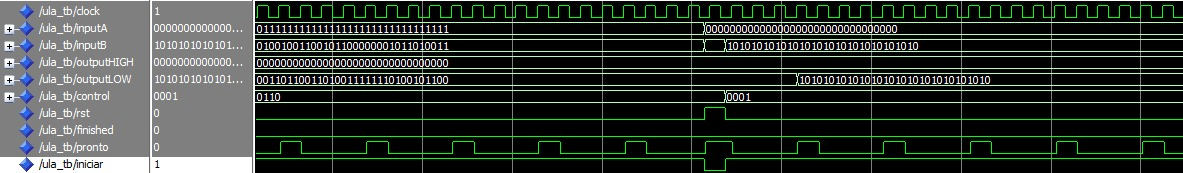
\includegraphics[scale=0.20]{testbench.jpeg}}
\caption{Verificação dos valores no testbench.}
\label{fig}
\end{figure}

A verificação das instruções padrão do MIPS ocorreram com os resultados esperados, evidenciando que seu funcionamento estava correto. Entretanto, a instrução de multiplicação apresentou erros em sua implementação, com valores de saída não esperados e não condizentes com as entradas sendo colocadas. Isso mostra que, no desenvolvimento do código, houve alguma falha na implementação da arquitetura da instrução, que acabou não funcionando corretamente, evidenciado pelos resultados do testbench.

\section{Resultados da síntese}
Devido ao número maior de bits de entrada e saída contido no MIPS, foi necessário escolher um FPGA diferente daquele utilizado ao longo da disciplina, que tivesse um número maior de pinos, e com isso, o Cyclone II EP2C35F672C6 foi escolhido. Esse FPGA conta com 475 pinos e 33.216 elementos lógicos, o que se mostrou suficiente para a aplicação desejada. O resultado da síntese no Quartus II é mostrado na figura a seguir.

\begin{figure}[htbp]
\centerline{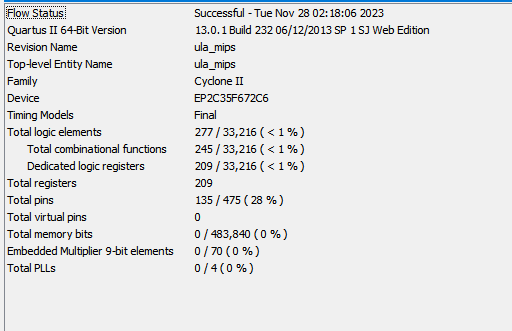
\includegraphics[scale=0.6]{io_report.png}}
\caption{Resultados da síntese da ULA 2.0.}
\label{fig}
\end{figure}

Ao rodar o TimeQuest para analisar os parâmetros de atraso e timing do projeto, um relatório foi gerado, o qual aponta uma frequência máxima de 184.13 MHz. Com isso, o período do clock é de aproximadamente 6ns.

\section{Conclusão}

O presente relatório apresenta uma proposta de melhoria na Unidade Lógica e Aritmética (ULA) da arquitetura MIPS, enfocando especificamente na instrução de multiplicação. A proposta de incrementar a capacidade de multiplicação demandou alterações substanciais na arquitetura original, abrangendo desde a modificação na largura dos bits de saída da ULA até ajustes nos componentes e na máquina de estados.

A adaptação na arquitetura foi conduzida de forma a comportar a instrução de multiplicação. A ampliação da saída da ULA para 64 bits, com divisão em registradores high e low de 32 bits, bem como a reconfiguração dos componentes para lidar com essa mudança, evidenciam a abordagem adotada. Os componentes fundamentais, como multiplexadores, registradores, operadores AND/OR e somadores/subtratores, foram devidamente ajustados para acomodar a nova instrução, com ênfase no somador e registradores de deslocamento adotados para a implementação da multiplicação.

A máquina de estados manteve similaridade com a ULA original, com a adição de estados específicos para a instrução de multiplicação. A descrição minuciosa dos estados relacionados à multiplicação, especialmente no que diz respeito ao ciclo de adições, contribui para a compreensão abrangente do funcionamento do sistema.

A análise dos resultados da síntese revela a necessidade de escolher um FPGA com maior capacidade, neste caso o Cyclone II EP2C35F672C6. Os números de pinos e elementos lógicos desse FPGA demonstraram-se adequados para a aplicação proposta, assegurando a viabilidade prática da arquitetura desenvolvida.

No plano de verificação, as instruções padrões do MIPS foram executadas da maneira esperada, com sucesso. Entretanto, a instrução sugerida de multiplicação não obteve os resultados esperados, ocorrendo erros na execução e valores de saída não condizentes.

Em suma, a abordagem para a implementação da instrução de multiplicação na ULA do MIPS, evidenciada neste relatório, não obteve o resultado esperado. A explicação detalhada da proposta, dos componentes ajustados e da máquina de estados, aliada à análise dos planos de verificação e dos resultados da síntese, proporciona uma visão abrangente do projeto, que pode abrir oportunidades da análise do que ocorreu de errado na implementação do projeto, e como modificá-lo para seu funcionamento completo a partir desse ponto.

\begin{thebibliography}{00}
\bibitem{b1} GHARRIS, David M.; HARRIS, Sarah L. Digital Design and Computer Architecture. Second edition. Waltham, MA, USA: Morgan Kaufmann Publishers, 2013. ISBN 978-0-12-394424-5
\bibitem{b2} PATTERSON, David A.; HENNESSY, John L. Organização e Projeto de Computadores: a interface hardware/software. Rio de Janeiro: Elsevier, 2005. ISBN 85-352-1521-2
\bibitem{b3} HU, Pong P. RTL Hardware Design Using VHDL: coding for efficiency, portability, and scalability. Hoboken, N.J.: Wiley-Interscience, 2006. ISBN 0471720925
\end{thebibliography}

\end{document}
